\chapter{Diseño e implementación}
\label{Chapter3}

Este capítulo describe la arquitectura y la organización interna del módulo de comunicación BLE desarrollado para el controlador N150. Se presenta su integración con el firmware existente, se detallan los módulos que componen \texttt{sfy-BLE} y se describe la configuración BLE implementada.

%----------------------------------------------------------------------------------------

\section{Arquitectura del sistema}
\label{sec:arquitectura_sistema}

El desarrollo se incorpora al firmware del N150 como el componente \texttt{sfy-BLE}. Su responsabilidad es proporcionar una interfaz de comunicación local basada en BLE para las tareas de soporte del controlador. El componente recibe solicitudes de un cliente BLE externo, las adapta a las interfaces disponibles en el firmware y publica las respuestas correspondientes. El cliente utiliza el módulo como servidor GATT, pero no forma parte del sistema desarrollado en este trabajo.

El alcance del trabajo se limita a \texttt{sfy-BLE}. Los subsistemas que gestionan el funcionamiento de la heladera, la persistencia de datos, los parámetros, la conectividad remota y los registros ya se encontraban desarrollados en el firmware del N150. Por este motivo, el módulo BLE no incorpora una segunda implementación de esas capacidades ni modifica sus responsabilidades. Su aporte consiste en habilitar un acceso local que reutiliza los servicios existentes.

La arquitectura general se organiza alrededor de \texttt{sfy-BLE}, destacado como el componente desarrollado, y de los módulos preexistentes del N150. La pila NimBLE provee el acceso a la radio y a los mecanismos BLE sobre los que se apoya \texttt{sfy-BLE}. A través de esta pila, el componente anuncia el equipo, atiende la conexión del cliente y administra la interfaz GATT.

Dentro de \texttt{sfy-BLE}, \texttt{ble-Main} administra el ciclo de vida de NimBLE. \texttt{ble-Gap} configura el \textit{advertising} y la conexión, mientras que \texttt{ble-Gatt} define los servicios y las características mediante los que se intercambian las solicitudes y respuestas con el cliente. Estos módulos constituyen la interfaz de comunicación local y coordinan el acceso a los módulos internos de procesamiento.

La figura \ref{fig:arquitectura_sistema} presenta los bloques principales y el flujo de procesamiento entre ellos. El recuadro exterior delimita el firmware del N150 y deja fuera al cliente BLE, que no forma parte del desarrollo. El recuadro de trazo grueso agrupa los módulos de \texttt{sfy-BLE}, y los bloques ubicados fuera de él corresponden a componentes preexistentes. Las líneas continuas indican intercambios directos y las punteadas, integraciones mediante callbacks.

\begin{figure}[!t]
\centering
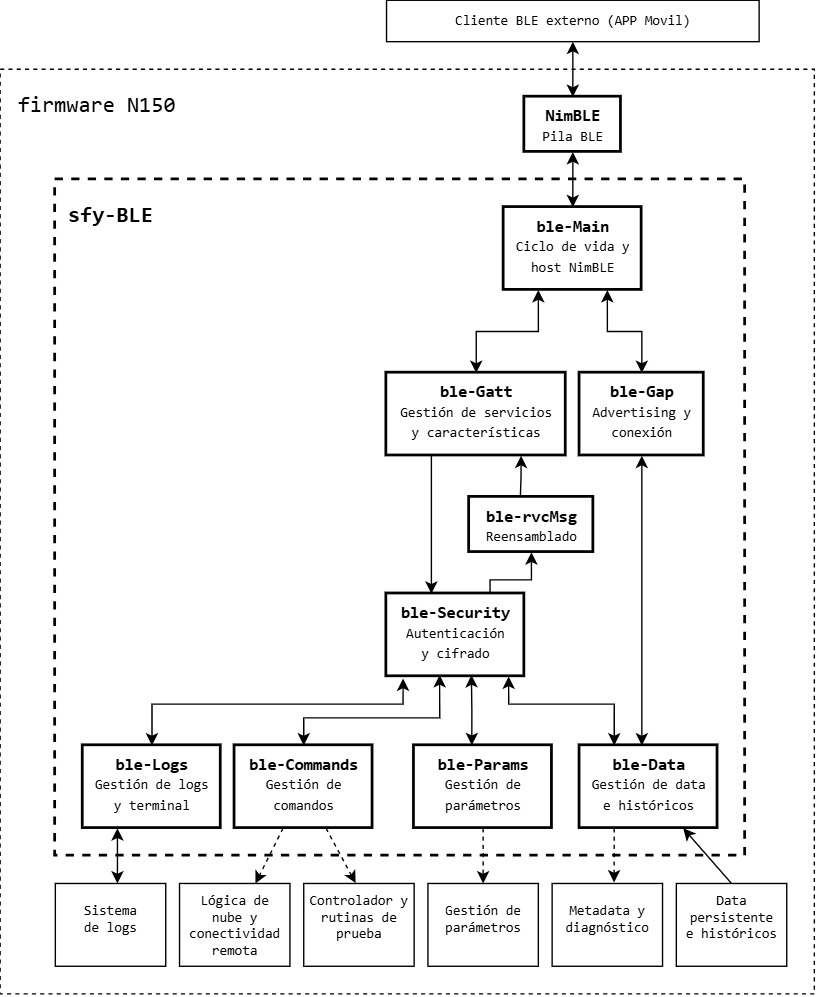
\includegraphics[width=\textwidth]{Figures/arquitecturaDiagrama2.png}
\caption{Arquitectura general del firmware N150 e integración del módulo \texttt{sfy-BLE}.}
\label{fig:arquitectura_sistema}
\end{figure}

\FloatBarrier

\subsection{Relación con los subsistemas del N150}

\texttt{sfy-BLE} se integra con el firmware mediante dos mecanismos distintos. El primero utiliza callbacks registrados durante la inicialización. Mediante estos callbacks, el módulo solicita la generación de metadatos y diagnóstico, la lectura y el procesamiento de parámetros, la ejecución de comandos locales y el encolado de comandos destinados a la lógica de nube y conectividad remota. Este mecanismo evita que \texttt{sfy-BLE} dependa directamente de las implementaciones internas de estos servicios.

La gestión de parámetros conserva, por lo tanto, las validaciones y el flujo de actualización que ya utilizaba el N150. De manera equivalente, las órdenes de control se resuelven mediante las rutinas existentes de prueba de los actuadores. Los comandos que deben alcanzar la infraestructura remota se entregan a la lógica de nube y conectividad remota para que sigan el mismo camino de procesamiento que los comandos recibidos por los medios de conectividad habituales.

El segundo mecanismo corresponde a dependencias directas del componente. \texttt{sfy-BLE} utiliza el subsistema de \textit{data} para obtener el último registro de telemetría y transferir el histórico almacenado. También se vincula con el sistema de registros para publicar mensajes generales y la salida de terminal durante una intervención de soporte. Estas dependencias forman parte de las operaciones internas de transferencia y depuración del módulo, por lo que no se exponen mediante callbacks del firmware principal.

La diferenciación entre ambos mecanismos responde al límite de responsabilidades definido para el desarrollo. Los callbacks se emplean cuando la operación pertenece a la lógica de negocio del N150 y debe permanecer controlada por el firmware principal. Las dependencias directas se emplean para los servicios que \texttt{sfy-BLE} necesita utilizar durante su funcionamiento interno. Esta decisión mantiene al componente desacoplado de las decisiones de control y conectividad, sin impedir el acceso a los datos y registros necesarios para la interfaz local.

\subsection{Flujo de procesamiento}

El flujo de procesamiento representado en la figura \ref{fig:arquitectura_sistema} es funcional y no corresponde a un diagrama estricto de llamadas entre archivos fuente. Las solicitudes recibidas por \texttt{ble-Gatt} que requieren fragmentación se entregan a \texttt{ble-rcvMsg}. Este módulo reensambla la secuencia recibida y, cuando completa el mensaje, lo entrega a \texttt{ble-Security}. El módulo de seguridad autentica la sesión, verifica el mensaje y recupera su contenido antes de que alcance los adaptadores funcionales.

Los módulos \texttt{ble-Commands}, \texttt{ble-Data} y \texttt{ble-Params} procesan el contenido validado según la operación solicitada. \texttt{ble-Logs} publica los registros generales y la salida de terminal utilizados durante soporte. Las operaciones de autenticación y los mensajes breves se procesan directamente entre \texttt{ble-Gatt} y \texttt{ble-Security}, sin requerir el reensamblado previo.

Una vez resuelta la solicitud, el resultado regresa a la interfaz GATT y se transmite al cliente BLE. Esta organización permite que la comunicación local sea una vía adicional de acceso al N150, sin alterar el funcionamiento interno de los módulos preexistentes. La arquitectura también facilita el mantenimiento: las modificaciones en los parámetros, el control o la lógica de nube y conectividad remota no requieren cambios en la capa BLE mientras se conserve el contrato de integración establecido.

%----------------------------------------------------------------------------------------

\section{Diseño detallado por módulos}
\label{sec:diseno_modulos}

La implementación se dividió en módulos con responsabilidades acotadas. La modularización combinó la separación de responsabilidades, la mantenibilidad y la posibilidad de realizar pruebas independientes. Esta organización evita concentrar la configuración de la pila, el procesamiento de mensajes, la seguridad y la integración con el N150 en un único componente. La tabla \ref{tab:modulos_ble} resume los módulos que conforman \texttt{sfy-BLE}.

\begin{table}[htbp]
\centering
\caption{Responsabilidades de los módulos del componente BLE.}
\label{tab:modulos_ble}
\begin{tabular}{p{0.25\textwidth} p{0.65\textwidth}}
\toprule
Módulo & Responsabilidad principal \\
\midrule
\texttt{ble-Main} & Administra el ciclo de vida de NimBLE, la tarea del host y la sincronización de los recursos compartidos. \\
\texttt{ble-Gap} & Configura el nombre, el \textit{advertising}, la conexión, la desconexión y la unidad máxima de transmisión (MTU, del inglés, \textit{Maximum Transmission Unit}). \\
\texttt{ble-Gatt} & Define servicios y características, procesa accesos y transmite notificaciones e indicaciones. \\
\texttt{ble-rcvMsg} & Reensambla mensajes fragmentados y valida secuencia, longitud y CRC32. \\
\texttt{ble-Security} & Implementa autenticación, claves de sesión, contadores y cifrado AES-256-GCM. \\
\texttt{ble-Data} & Genera metadatos, diagnóstico e histórico, y administra los datos de \textit{advertising}. \\
\texttt{ble-Params} & Vincula las solicitudes de lectura y escritura con el gestor de parámetros. \\
\texttt{ble-Commands} & Adapta los comandos locales y los destinados a la lógica de nube y conectividad remota. \\
\texttt{ble-Logs} & Publica registros generales y la salida de terminal para soporte y depuración. \\
\bottomrule
\end{tabular}
\end{table}

\subsection{\texttt{ble-Main}}

\texttt{ble-Main} administra el ciclo de vida de la pila NimBLE mediante cuatro estados: detenido, iniciando, iniciado y deteniendo. Las transiciones se protegen con un mutex recursivo compartido con \texttt{ble-Params}. El carácter recursivo permite que un cambio del modo de operación, que ya retiene el mutex, invoque el inicio o la detención de la pila sin bloquearse a sí mismo. Las solicitudes que coinciden con el estado actual se resuelven sin efectos, mientras que las que llegan durante una transición en curso se rechazan, de modo que no se reinicializan recursos que puedan estar en uso.

La inicialización recibe el serial del equipo, prepara el material criptográfico utilizado por \texttt{ble-Security} y, si el parámetro \texttt{APP\_LINK} no deshabilita la interfaz, inicia la pila. El inicio construye el nombre publicado a partir del serial, inicializa NimBLE y los servicios del perfil de acceso genérico (GAP, del inglés, \textit{Generic Access Profile}) y GATT, registra los callbacks del host y crea una tarea de FreeRTOS dedicada a ejecutar el host BLE. Esta tarea separa el procesamiento de eventos BLE del flujo principal del firmware. Si alguna de estas etapas falla, se libera lo ya inicializado y el estado vuelve a detenido. El \textit{advertising} no comienza durante el inicio, sino cuando el host se sincroniza con el controlador. En ese momento se fija una MTU preferida de 256 bytes y se delega a \texttt{ble-Gap} la configuración del \textit{advertising}.

La detención sigue el orden inverso. Primero se detiene el \textit{advertising} y se cierra la conexión activa, luego se solicita la finalización del host y se espera que su tarea termine antes de liberar la pila. Si la tarea no finaliza dentro del tiempo previsto o la liberación falla, el módulo conserva el estado iniciado y no informa una detención incompleta como exitosa. Los parámetros con los que se configura la pila se describen en la sección \ref{sec:configuracion_ble}.

\subsection{\texttt{ble-Gap} y \texttt{ble-Gatt}}

\texttt{ble-Gap} concentra los procedimientos de descubrimiento y conexión. Construye el nombre del equipo a partir de su serial, configura los datos de \textit{advertising} y responde a los eventos de conexión, desconexión y negociación de MTU. Al finalizar una conexión, restablece el estado necesario para que el controlador vuelva a estar disponible para una nueva intervención local. Las decisiones de diseño de esta capa se describen en la sección \ref{sec:diseno_gap}.

\texttt{ble-Gatt} define la interfaz de servicios y características utilizada por el cliente BLE. Sus manejadores reciben las operaciones de lectura, escritura y suscripción, y coordinan la transmisión de notificaciones e indicaciones. También constituye el punto de integración con \texttt{ble-rcvMsg}, \texttt{ble-Security} y los adaptadores funcionales. Esta división permite modificar la estructura GATT sin incorporar en sus manejadores la lógica de reensamblado, autenticación o acceso a los subsistemas del N150. Las decisiones de diseño de esta capa se describen en la sección \ref{sec:diseno_gatt}.

\subsection{\texttt{ble-rcvMsg} y \texttt{ble-Security}}

\texttt{ble-rcvMsg} se separó de la capa GATT para reutilizar la fragmentación y sus validaciones en las características que reciben mensajes extensos. El módulo reensambla la secuencia recibida y verifica número de secuencia, longitud y CRC32 antes de entregar el mensaje completo. De este modo, los manejadores GATT permanecen enfocados en el acceso a las características y no replican el tratamiento de cada fragmento.

\texttt{ble-Security} implementa una política transversal para todas las operaciones funcionales. Administra la autenticación de sesión, las claves temporales, los contadores y el cifrado de mensajes. Mantener esta función en un módulo separado evita mezclar detalles criptográficos con los servicios GATT y permite modificar el mecanismo de protección sin alterar los adaptadores de datos, parámetros o comandos.

\subsection{\texttt{ble-Data} y \texttt{ble-Params}}

\texttt{ble-Data} concentra las operaciones de consulta. Genera metadatos del equipo, un diagnóstico de conectividad y la transferencia de información histórica almacenada. Los metadatos y el diagnóstico se obtienen mediante callbacks, mientras que el histórico y el último registro de telemetría se integran con el subsistema de \textit{data}. El último registro también se entrega a \texttt{ble-Gap} para el modo de \textit{advertising} con datos.

\texttt{ble-Params} atiende la consulta y el procesamiento de cambios de configuración. Ambas operaciones se delegan mediante callbacks al gestor de parámetros ya existente. Luego de una modificación, el firmware conserva su mecanismo habitual de reporte de cambios, de modo que la interfaz local no introduce un flujo de configuración paralelo.

\subsection{\texttt{ble-Commands} y \texttt{ble-Logs}}

\texttt{ble-Commands} diferencia las acciones locales de control de los comandos destinados a la infraestructura remota. Las acciones locales se delegan mediante un callback a las rutinas existentes del controlador. Los comandos remotos se incorporan a la cola de la lógica de nube y conectividad remota, lo que evita duplicar validaciones y conserva el flujo normal de procesamiento.

\texttt{ble-Logs} ofrece canales para registros generales y salida de terminal. Esta capacidad se utilizó durante el desarrollo para depurar la interfaz BLE y durante soporte para observar el comportamiento del N150 sin depender de la conectividad celular. El módulo limita la tasa de envío y conserva los mensajes de terminal en un búfer circular, con el objetivo de que la depuración no interfiera con las operaciones funcionales de la interfaz local.

%----------------------------------------------------------------------------------------

\section{Configuración BLE implementada}
\label{sec:configuracion_ble}

ESP-IDF agrupa la configuración de Bluetooth en un conjunto de opciones que se seleccionan mediante la herramienta de configuración del proyecto y se almacenan en el archivo \texttt{sdkconfig}. Estas opciones se organizan en tres niveles: la habilitación de Bluetooth y la selección de la pila del host, los parámetros del host elegido y los parámetros del controlador de radio. Cada opción tiene un valor por defecto definido por ESP-IDF. Para \texttt{sfy-BLE} se partió de esos valores y se modificaron únicamente los que no se correspondían con el uso previsto de la interfaz local. Esta sección describe las opciones disponibles, los valores por defecto de ESP-IDF 5.3.2 y los cambios realizados.

\subsection{Selección de la pila y del controlador}
\label{subsec:config_pila}

ESP-IDF ofrece dos implementaciones del host Bluetooth \cite{espressif:esp-idf-ble}. Bluedroid, la opción por defecto, admite tanto Bluetooth clásico como BLE. NimBLE implementa únicamente BLE y requiere menos memoria y menos espacio de programa. También es posible habilitar solo el controlador, para los casos en que el host se ejecuta en otro procesador. Como la interfaz local utiliza exclusivamente BLE, se reemplazó Bluedroid por NimBLE. De este modo, el firmware no incorpora el soporte de Bluetooth clásico, que no se utiliza y ocuparía recursos compartidos con el resto de los subsistemas del N150.

El controlador del ESP32 puede operar en modo BLE, en modo Bluetooth clásico o en modo dual. Se mantuvo el valor por defecto, que habilita solo BLE y es coherente con la pila elegida. El ESP32 implementa la especificación Bluetooth 4.2 \cite{espressif:esp32}, por lo que ESP-IDF no habilita las funciones de Bluetooth 5, como el \textit{advertising} extendido. En consecuencia, cada paquete de \textit{advertising} del N150 admite como máximo 31 bytes, restricción que condiciona el diseño de la capa GAP.

\subsection{Opciones del host NimBLE}
\label{subsec:config_nimble}

Las opciones de NimBLE abarcan, entre otras, los roles habilitados, la cantidad de conexiones simultáneas, la memoria reservada para los mensajes de la pila, la MTU preferida y el nivel de registros. Los valores por defecto están pensados para un uso general, en el que el dispositivo puede actuar a la vez como central y como periférico y mantener varias conexiones. El N150 cumple un rol más acotado: actúa solo como periférico y atiende a un único teléfono por vez. Por este motivo, se deshabilitaron los roles innecesarios y se redujeron las reservas de memoria, que en el ESP32 se comparten con el resto de los subsistemas del firmware. La tabla \ref{tab:config_nimble} resume las opciones revisadas, con su valor por defecto, el valor adoptado y el motivo de cada elección.

\begin{table}[htbp]
\centering
\caption{Opciones del host NimBLE revisadas.}
\label{tab:config_nimble}
\small
\setlength{\tabcolsep}{4pt}
\begin{tabular}{L{0.24\textwidth} L{0.15\textwidth} L{0.17\textwidth} L{0.32\textwidth}}
\toprule
Opción & Valor por defecto & Valor adoptado & Motivo \\
\midrule
Conexiones simultáneas & 3 & 1 & La interfaz local atiende a un único teléfono. \\
Rol periférico & Habilitado & Habilitado & Permite anunciar el equipo y aceptar conexiones. \\
Roles central y \textit{broadcaster} & Habilitados & Deshabilitados & El equipo no inicia conexiones y el \textit{advertising} conectable forma parte del rol periférico. \\
Bloques de memoria del primer grupo & 12 $\times$ 256~B & 12 $\times$ 256~B & Resultan suficientes para el tráfico de la interfaz local. \\
Bloques de memoria del segundo grupo & 24 $\times$ 320~B & Ninguno & Los mensajes extensos se fragmentan en la capa de aplicación. \\
Búferes de datos entrantes & 24 $\times$ 255~B & 8 $\times$ 255~B & El tráfico entrante desde el teléfono es reducido. \\
MTU preferida & 256~B & 256~B & Coincide con la solicitada por la aplicación móvil. \\
Nivel de registros de la pila & Información & Advertencia & Limita los mensajes de NimBLE a advertencias y errores. \\
Ubicación de la memoria del host & Interna & PSRAM & Libera memoria interna (sección \ref{subsec:config_psram}). \\
Nombre GAP por defecto & \texttt{nimble} & \texttt{nimble} & \texttt{sfy-BLE} lo reemplaza durante el inicio por un nombre basado en el serial. \\
\bottomrule
\end{tabular}
\end{table}

Para cuantificar el efecto de estos ajustes se midió la memoria libre antes y después de iniciar la pila. Con la configuración utilizada al comienzo del desarrollo, que admitía tres conexiones, mantenía todos los roles y reservaba más bloques de memoria, la pila consumía 43\,740 bytes. Con la configuración adoptada, el consumo se redujo a 13\,980 bytes, lo que liberó 29\,760 bytes para el resto del firmware.

\texttt{sfy-BLE} incluye un archivo con los valores de configuración que requiere, para que el proyecto que lo integra los incorpore a su propio \texttt{sdkconfig}. Además, la configuración se verifica durante la compilación. Si el proyecto no habilita BLE y NimBLE, o define una MTU o una cantidad de conexiones distintas de las esperadas, la compilación se interrumpe con un mensaje que indica el valor que debe corregirse. Este control evita que una diferencia de configuración se manifieste recién durante la operación del equipo.

\subsection{Uso de memoria externa}
\label{subsec:config_psram}

Como se indicó en la sección \ref{sec:controlador_n150}, el ESP32 del N150 dispone de 2~MB de PSRAM. Hasta la incorporación de la interfaz BLE, el firmware no utilizaba esta memoria.

La pila Bluetooth de Espressif ocupa memoria interna en dos partes. El controlador reserva de forma fija 56\,156 bytes de la RAM interna, que no pueden ubicarse en la memoria externa. Al iniciarse, el host asigna además sus estructuras y búferes de forma dinámica, que con la configuración adoptada ocupan los 13\,980 bytes medidos. Con todas estas asignaciones en la memoria interna, el ESP32 no disponía de memoria suficiente para ejecutar la pila junto con los subsistemas preexistentes del N150.

Para resolverlo, se habilitó la PSRAM y se configuró NimBLE para asignar su memoria en ella. ESP-IDF ofrece cuatro estrategias de asignación para el host: memoria interna, que es la opción por defecto, memoria externa, la estrategia general del sistema y la RAM de instrucciones interna. Se eligió la memoria externa, de modo que la memoria interna queda disponible para el controlador y para el resto del firmware.

%----------------------------------------------------------------------------------------

\section{Diseño de la capa GAP}
\label{sec:diseno_gap}

La capa GAP determina cómo el N150 se da a conocer a los teléfonos cercanos y cómo se establece la conexión. Su diseño partió de dos condiciones definidas en la sección \ref{sec:configuracion_ble}: el equipo actúa solo como periférico y cada paquete de \textit{advertising} admite como máximo 31 bytes. Dentro de ese marco, se buscó que el equipo pudiera encontrarse en cualquier momento sin intervención sobre el controlador, que su comportamiento pudiera adaptarse a cada cliente y que parte de su información pudiera consultarse sin establecer una conexión.

\subsection{Identificación del equipo}
\label{subsec:gap_identificacion}

El equipo se identifica mediante su dirección BLE y su nombre. Como dirección se utiliza la dirección pública que el ESP32 trae asignada de fábrica, por lo que un mismo controlador conserva siempre la misma identidad.

El nombre publicado se forma con el prefijo \texttt{sfy} seguido del serial del equipo. El prefijo permite que la aplicación filtre los controladores de Sensify entre todos los dispositivos BLE presentes en el lugar, y el serial permite que el técnico reconozca el equipo sobre el que debe intervenir sin necesidad de conectarse. El nombre se asigna durante el inicio de la pila y reemplaza el nombre genérico configurado en ESP-IDF.

\subsection{Contenido del \textit{advertising}}
\label{subsec:gap_contenido}

El N150 publica paquetes de \textit{advertising} conectables y no dirigidos, con descubrimiento general e indicación de que no admite Bluetooth clásico. El \textit{advertising} no tiene tiempo límite. Se mantiene mientras no haya un teléfono conectado y se reanuda cuando la conexión finaliza, cuando un intento de conexión falla o cuando la pila informa su interrupción. De este modo, el equipo puede descubrirse en cualquier momento sin que el técnico deba realizar una acción previa sobre el controlador.

El límite de 31 bytes por paquete fue una de las principales dificultades del diseño de esta capa. Como el ESP32 implementa Bluetooth 4.2, no dispone del \textit{advertising} extendido de Bluetooth 5, que admite paquetes de mayor tamaño. En el paquete principal, los indicadores de descubrimiento ocupan 3 bytes y el campo con el registro de telemetría, 26 bytes. Quedan entonces solo 2 bytes libres, insuficientes para incluir también el nombre del equipo.

Para resolverlo, se utilizó el \textit{scan response}, un segundo paquete de hasta 31 bytes que el periférico entrega cuando el teléfono lo solicita mediante un \textit{scan request} durante el escaneo. El contenido se repartió entre ambos paquetes, como resume la tabla \ref{tab:contenido_adv}. El paquete principal transporta los indicadores de descubrimiento y, cuando el modo de operación lo requiere, los datos de telemetría. El \textit{scan response} transporta solo el nombre completo, de modo que su longitud no reduce el espacio disponible para los datos. El teléfono recibe ambos paquetes y los asocia al mismo equipo mediante su dirección.

\begin{table}[htbp]
\centering
\caption{Distribución del contenido del \textit{advertising}.}
\label{tab:contenido_adv}
\begin{tabular}{L{0.22\textwidth} L{0.30\textwidth} L{0.12\textwidth} L{0.23\textwidth}}
\toprule
Paquete & Campo & Tamaño & Presencia \\
\midrule
\textit{Advertising} & Indicadores de descubrimiento & 3~B & Siempre. \\
 & Datos específicos del fabricante & 26~B & Solo en el modo con datos. \\
\textit{Scan response} & Nombre completo del equipo & Variable & Según el modo. \\
\bottomrule
\end{tabular}
\end{table}

\subsection{Modos de operación}
\label{subsec:gap_modos}

Las instalaciones del N150 no tienen todas las mismas necesidades. Por este motivo, el comportamiento de la capa GAP se definió como configurable mediante el parámetro \texttt{APP\_LINK}, administrado por el gestor de parámetros del equipo. Al ser un parámetro más del N150, puede ajustarse para cada cliente por los mismos medios que el resto de la configuración. La tabla \ref{tab:modos_app_link} resume los cuatro modos disponibles.

\begin{table}[htbp]
\centering
\caption{Modos de operación definidos por \texttt{APP\_LINK}.}
\label{tab:modos_app_link}
\begin{tabular}{L{0.26\textwidth} L{0.22\textwidth} L{0.20\textwidth} L{0.19\textwidth}}
\toprule
Modo & Datos en el \textit{advertising} & Nombre en el \textit{scan response} & Intervalo de \textit{advertising} \\
\midrule
Deshabilitado & \multicolumn{3}{l}{Pila BLE detenida.} \\
\textit{Advertising} con datos y conexión & Último registro de telemetría & Sí & 500--510~ms \\
\textit{Advertising} y conexión (predeterminado) & No & Sí & 500--510~ms \\
Solo conexión & No & No & 2000--3000~ms \\
\bottomrule
\end{tabular}
\end{table}

El modo predeterminado corresponde al uso más general: el equipo se anuncia con su nombre cada medio segundo, lo que permite que la aplicación lo encuentre rápidamente y que el técnico se conecte. El modo de solo conexión mantiene el equipo conectable, pero no publica su nombre y espacia los anuncios entre 2 y 3~s. Así se reduce su visibilidad para quienes exploran los dispositivos cercanos y disminuye la actividad de la radio. El modo deshabilitado detiene la pila para las instalaciones que no requieren la interfaz local.

Un cambio de modo se aplica sin reiniciar el equipo. Si se deshabilita la interfaz, se detiene la pila; si se habilita, se inicia; y si se pasa de un modo activo a otro, solo se actualiza el contenido del \textit{advertising}, sin interrumpir la publicación.

\subsection{\textit{Advertising} con datos}
\label{subsec:gap_adv_datos}

La conexión con el equipo requiere que el técnico la inicie desde la aplicación y que se complete la autenticación antes de acceder a la información. Este proceso resulta adecuado para configurar o diagnosticar un controlador en particular, pero es lento cuando solo se necesita una visión rápida del estado de varios equipos. El modo con datos se diseñó para ese caso. Al incluir la última medición en el \textit{advertising}, la aplicación puede mostrar el estado de todas las heladeras cercanas con solo explorar el entorno, a modo de \textit{display} virtual, sin que el técnico deba conectarse, autenticarse ni interactuar con cada equipo. La figura \ref{fig:display_virtual} muestra el \textit{display} virtual de una heladera en la aplicación móvil. En él, las temperaturas, el estado de la puerta y de las salidas, la tensión medida, las alarmas, el tipo de red y la intensidad de señal provienen del \textit{advertising}; los valores restantes no forman parte de él.

\begin{figure}[htbp]
\centering
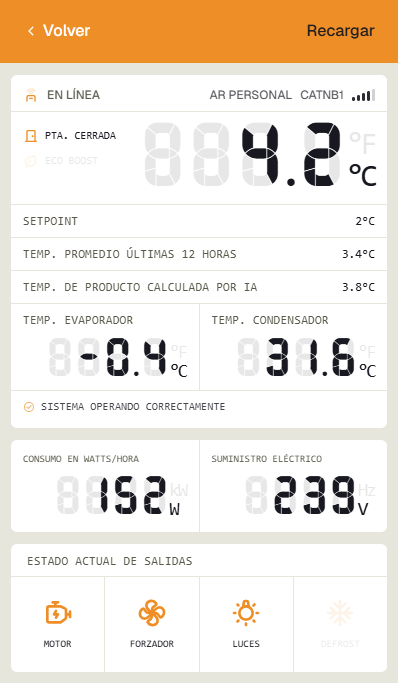
\includegraphics[width=0.38\textwidth]{Figures/displayVirtual.png}
\caption{\textit{Display} virtual de una heladera en la aplicación móvil.}
\label{fig:display_virtual}
\end{figure}

Los datos se transmiten en el campo de datos específicos del fabricante. Su contenido es el último registro de telemetría, que \texttt{ble-Data} obtiene del subsistema de \textit{data} y codifica con el mismo formato binario que el equipo utiliza para enviar la telemetría a la plataforma de Sensify. El registro incluye el tipo de red y la intensidad de señal, las temperaturas interna, del evaporador y del condensador, la tensión de alimentación, la marca de tiempo, indicadores del estado de la puerta, de las salidas y de las alarmas, y una suma de verificación. Codificado, ocupa 23 bytes, por lo que entra completo en el campo de 24 bytes disponible luego de los indicadores de descubrimiento. La reutilización de este formato evitó definir una codificación adicional para la interfaz local.

El contenido se actualiza cada vez que se inicia el \textit{advertising} y cada vez que se modifica sin detenerlo. En ambos casos, \texttt{ble-Gap} solicita el registro más reciente a \texttt{ble-Data} y reemplaza el campo solo si la información cambió.

La figura \ref{fig:flujo_adv_datos} resume el flujo completo del modo con datos, desde la obtención del registro hasta su visualización en la aplicación móvil.

\begin{figure}[htbp]
\centering
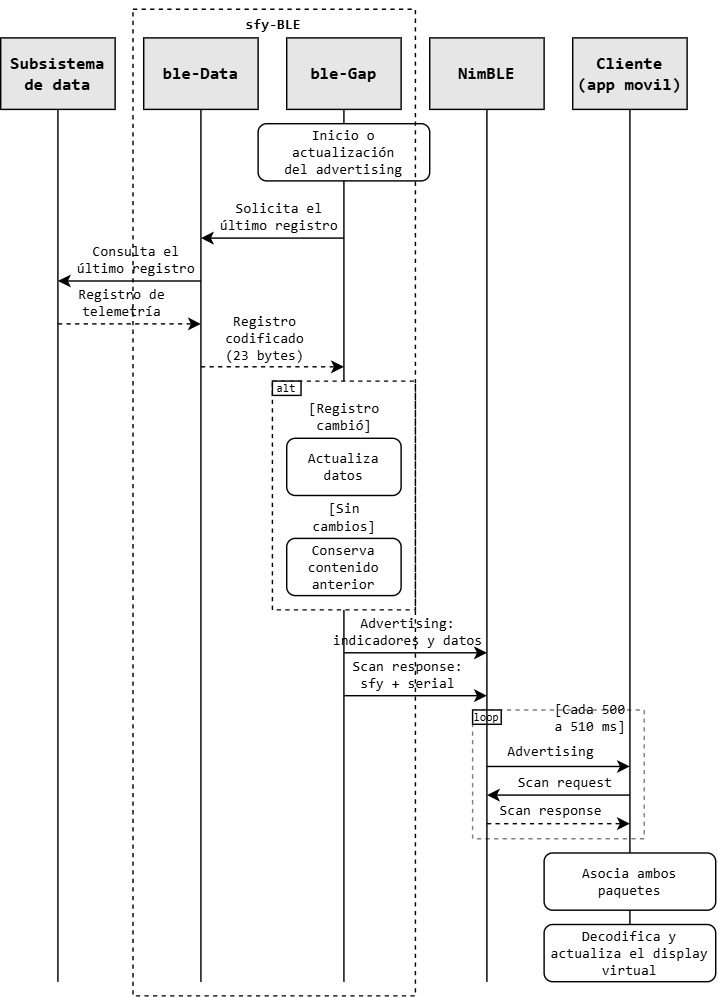
\includegraphics[width=0.85\textwidth]{Figures/flujoAdvDatos.jpg}
\caption{Flujo del \textit{advertising} con datos.}
\label{fig:flujo_adv_datos}
\end{figure}

\subsection{Gestión de la conexión}
\label{subsec:gap_conexion}

El equipo admite una única conexión, de modo que un solo teléfono opera el N150 por vez. Al establecerse la conexión, el \textit{advertising} se detiene, por lo que el controlador deja de aparecer para otros teléfonos hasta que la sesión finaliza.

Luego de conectarse, el N150 solicita conservar el intervalo de conexión y el tiempo de supervisión propuestos por el teléfono, con una latencia de periférico de tres eventos. La latencia permite que el equipo omita hasta tres eventos de conexión consecutivos cuando no tiene datos para transmitir. De este modo, se estabiliza la conexión y se reduce la actividad de la radio sin modificar los tiempos negociados por el teléfono. La MTU preferida es de 256 bytes, y el valor efectivo surge de la negociación que el teléfono realiza al conectarse.

Al finalizar la conexión, \texttt{ble-Gap} descarta la sesión segura y cualquier mensaje recibido de forma parcial, y reanuda el \textit{advertising} salvo que la interfaz haya sido deshabilitada. Esta limpieza garantiza que cada sesión comience desde un estado conocido y que la información de una sesión anterior no se reutilice en la siguiente.

%----------------------------------------------------------------------------------------

\section{Diseño de la capa GATT}
\label{sec:diseno_gatt}

La capa GATT define la interfaz mediante la cual la aplicación móvil accede a las funciones del N150 una vez establecida la conexión. Su diseño persiguió tres objetivos: organizar las operaciones por área funcional, transferir respuestas que superan el tamaño de un paquete sin perder información y facilitar la incorporación de nuevas funciones sin modificar la estructura existente.

\subsection{Organización de servicios y características}
\label{subsec:gatt_organizacion}

La interfaz se organiza en cuatro servicios primarios: control, datos, parámetros y depuración. Cada servicio agrupa las características de un área funcional, como resume la tabla \ref{tab:servicios_gatt}.

\begin{table}[!h]
\centering
\caption{Servicios y características GATT implementados.}
\label{tab:servicios_gatt}
\footnotesize
\setlength{\tabcolsep}{4pt}
\begin{tabular}{L{0.12\textwidth} L{0.27\textwidth} L{0.14\textwidth} L{0.37\textwidth}}
\toprule
Servicio & Característica & Propiedad & Uso \\
\midrule
Control & \texttt{AUTH-SYNC} & Lectura y escritura & Establecimiento de la sesión segura. \\
 & \texttt{COMMAND-GET} & Escritura & Comandos de control local. \\
 & \texttt{COMMANDS-RESPONSE} & Notificación & Estado de los comandos de control. \\
 & \texttt{CLOUDCOMMANDS-GET} & Escritura & Comandos para la lógica de nube y conectividad remota. \\
 & \texttt{LOG-CONTROL} & Notificación & Eventos y estado de procesos. \\
\midrule
Datos & \texttt{TIME-SYNC} & Escritura & Sincronización de fecha y hora. \\
 & \texttt{COMMAND-DATA} & Escritura & Solicitudes de metadatos, diagnóstico, histórico y parámetros. \\
 & \texttt{METADATA-READ} & Indicación & Metadatos del equipo. \\
 & \texttt{HISTORY-SEND} & Indicación & Registros históricos. \\
 & \texttt{DIAGNOSIS-READ} & Indicación & Diagnóstico de conectividad. \\
 & \texttt{READ-STATUS} & Notificación & Estado de las lecturas en curso. \\
\midrule
Parámetros & \texttt{PARAMETROS-GET} & Escritura & Envío de cambios de configuración. \\
 & \texttt{PARAMETROS-RESPONSE} & Indicación & Respuesta del gestor de parámetros. \\
\midrule
Depuración & \texttt{LOG-SEND} & Notificación & Registros generales. \\
 & \texttt{LOG-TERMINAL} & Notificación & Salida de terminal. \\
\bottomrule
\end{tabular}
\end{table}

Salvo en el establecimiento de la sesión, la interfaz no utiliza lecturas GATT directas. Cada operación combina una característica de escritura, por la que la aplicación envía la solicitud, con otra de indicación o notificación, por la que el equipo entrega la respuesta. Esta separación responde a dos motivos. En primer lugar, muchas respuestas, como los metadatos, el diagnóstico o la configuración, superan el tamaño de un paquete y se generan de forma asincrónica, por lo que el equipo las envía cuando están listas y fragmentadas. En segundo lugar, las indicaciones requieren que la aplicación confirme cada recepción, lo que garantiza que un fragmento llegó antes de enviar el siguiente.

\subsection{Diseño orientado a la extensión}
\label{subsec:gatt_extension}

La estructura GATT se diseñó para que incorporar un servicio o una característica no requiera modificar la lógica existente. Con este fin, se combinaron cuatro decisiones.

La primera es la definición declarativa de la interfaz. Los servicios y las características se describen en una única tabla, en la que cada característica es una entrada con su identificador, sus propiedades y la función que atiende sus accesos. NimBLE recorre esa tabla durante el inicio y registra la estructura completa, por lo que agregar una característica consiste en agregar una entrada.

El código \ref{lst:tabla_gatt} muestra un fragmento de la tabla con el servicio de datos y dos de sus características. Cada característica se define con su identificador, la función que atiende sus accesos, sus propiedades y la variable en la que NimBLE guarda su \textit{handle}.
\begin{lstlisting}[float=!htbp, caption={Fragmento de la tabla de servicios GATT.}, label=lst:tabla_gatt]
static const struct ble_gatt_svc_def gatt_services[] = {
    {   /* Servicio de datos */
        .type = BLE_GATT_SVC_TYPE_PRIMARY,
        .uuid = &data_svc_uuid.u,
        .characteristics = (struct ble_gatt_chr_def[]) {
            {   /* COMMAND-DATA: solicitudes de la aplicación */
                .uuid       = &commandData_chr_uuid.u,
                .access_cb  = commandData_access_cb,
                .flags      = BLE_GATT_CHR_F_WRITE,
                .val_handle = &commandData_handle,
            },
            {   /* METADATA-READ: respuesta por indicación */
                .uuid       = &metadataRead_chr_uuid.u,
                .access_cb  = metadataRead_access_cb,
                .flags      = BLE_GATT_CHR_F_INDICATE,
                .val_handle = &g_metadataRead.attr_handle,
            },
            { 0 },  /* fin de las características */
        }
    },
    /* ... servicios de control, parámetros y depuración ... */
    { 0 },  /* fin de los servicios */
};
\end{lstlisting}

La segunda es un esquema de identificadores con base común. Los servicios y las características se identifican mediante identificadores únicos universales (UUID, del inglés, \textit{Universally Unique Identifier}) de 128 bits que comparten una base propia de Sensify y difieren solo en el primer byte. Dentro de ese byte, la parte alta identifica el servicio y la parte baja, la característica: el servicio de control utiliza el valor \texttt{0xF0} y sus características, los valores \texttt{0xF1} a \texttt{0xF5}. Un servicio nuevo toma el siguiente prefijo libre y una característica nueva, el siguiente valor dentro de su servicio.

La tercera es la separación entre la definición de una característica y su mecanismo de transmisión. Las indicaciones y las notificaciones se gestionan mediante dos mecanismos genéricos, descritos en la sección \ref{subsec:gatt_transmision}, que resuelven la suscripción, la fragmentación, los reintentos y el control de tasa. Cada característica que transmite datos solo declara un contexto con la función que entrega el próximo mensaje. En la tabla de servicios, el \textit{handle} de esa característica se guarda dentro de su contexto, como ocurre con \texttt{g\_metadataRead} en el código \ref{lst:tabla_gatt}, lo que la vincula con el mecanismo correspondiente. La suscripción también se atiende de forma genérica: el manejador identifica la característica por su \textit{handle} y actualiza su contexto, sin lógica específica para cada caso.

La cuarta es el uso de comandos binarios sobre características compartidas, descritos en la sección \ref{subsec:gatt_comandos}. Una operación nueva sobre un servicio existente puede incorporarse como un nuevo código de comando, sin crear una característica adicional.

\subsection{Comandos, estados y formatos}
\label{subsec:gatt_comandos}

Las solicitudes breves se envían como comandos binarios: un código de 2 bytes seguido de un argumento opcional de 1 byte. Los códigos se agruparon por rangos según el tipo de operación, como resume la tabla \ref{tab:comandos_gatt}. \texttt{COMMAND-DATA} recibe las consultas y \texttt{COMMAND-GET}, las acciones de control.

\begin{table}[htbp]
\centering
\caption{Comandos binarios de la interfaz GATT.}
\label{tab:comandos_gatt}
\small
\begin{tabular}{L{0.14\textwidth} L{0.36\textwidth} L{0.38\textwidth}}
\toprule
Código & Comando & Operación \\
\midrule
\texttt{0x0001} & \texttt{CMD\_METADATA\_READ} & Lectura de metadatos. \\
\texttt{0x0002} & \texttt{CMD\_CONNECTIVITY\_READ} & Lectura del diagnóstico de conectividad. \\
\midrule
\texttt{0x1000} & \texttt{CMD\_HISTORY\_GET} & Inicio de la descarga del histórico. \\
\texttt{0x1001} & \texttt{CMD\_HISTORY\_CONFIRM} & Confirmación de la descarga. \\
\texttt{0x1002} & \texttt{CMD\_HISTORY\_CANCEL} & Cancelación de la descarga. \\
\texttt{0x1003} & \texttt{CMD\_PARAMS\_READ} & Lectura de la configuración actual. \\
\midrule
\texttt{0x3010}--\texttt{0x3015} & \texttt{CMD\_CTRL\_TEST\_*} & Pruebas de compresor, resistencia, ventilador, luz y rutina completa. \\
\bottomrule
\end{tabular}
\end{table}

Las operaciones asincrónicas informan su avance mediante un mensaje de estado uniforme de 3 bytes, formado por el código del comando y un valor de estado: correcto, en curso o un código de error. Las lecturas lo publican en \texttt{READ-STATUS} y las acciones de control, en \texttt{COMMANDS-RESPONSE}. De este modo, la aplicación conoce en todo momento si una operación fue aceptada, si sigue en curso o si falló, con el mismo formato para todas las operaciones. Si llega una solicitud mientras la misma transferencia está en curso, se rechaza con un estado de ocupado, en lugar de interrumpir la transferencia anterior.

Los formatos se eligieron según el tamaño y la estructura de cada mensaje. Los comandos y los estados utilizan el formato binario descrito, por su brevedad. Los parámetros, los metadatos, el diagnóstico y los comandos para la lógica de nube y conectividad remota utilizan JSON, que se fragmenta cuando supera el tamaño de un paquete. Se mantuvo este formato porque es el que ya utilizaban los canales de conectividad remota existentes, lo que permitió reutilizar el procesamiento del firmware sin conversiones adicionales. Los registros históricos conservan el formato binario de la telemetría que el equipo envía a la plataforma. Por último, los canales de depuración no requieren comandos: la transmisión de registros comienza cuando la aplicación se suscribe a la característica y se detiene cuando cancela la suscripción.

\subsection{Transmisión de respuestas}
\label{subsec:gatt_transmision}

Las respuestas que requieren confirmación se transmiten mediante indicaciones. El mecanismo de indicaciones divide el mensaje en fragmentos y envía cada uno solo después de recibir la confirmación del anterior. Si la entrega de un fragmento falla, se reintenta hasta cinco veces antes de abortar la transferencia e informar el error por el canal de estado. Cuando la característica dispone de una función que entrega el próximo mensaje, el mecanismo la invoca al completar cada envío, lo que permite transmitir secuencias de mensajes sin cargarlas completas en memoria.

Los mensajes que superan el tamaño de un paquete se dividen en fragmentos. Cada fragmento comienza con un encabezado de texto, seguido de la porción del mensaje que transporta:

\begin{center}
\texttt{SEQ=<seq>;N=<total>;LEN=<len>;CRC=<crc>;F=<flag>;<payload>}
\end{center}

La tabla \ref{tab:trama_fragmento} describe cada campo. El formato es el mismo en ambos sentidos: \texttt{ble-rcvMsg} lo valida al recibir y \texttt{ble-Gatt} lo genera al transmitir. En el sentido del equipo hacia el teléfono, el contenido de cada fragmento se limita a 128 bytes.

\begin{table}[htbp]
\centering
\caption{Campos de la trama de fragmentación.}
\label{tab:trama_fragmento}
\begin{tabular}{L{0.14\textwidth} L{0.74\textwidth}}
\toprule
Campo & Contenido \\
\midrule
\texttt{SEQ} & Número de secuencia del fragmento. Comienza en 0 y aumenta de a uno. \\
\texttt{N} & Cantidad total de fragmentos del mensaje. \\
\texttt{LEN} & Longitud total del mensaje completo, en bytes. \\
\texttt{CRC} & CRC32 del mensaje completo, sin los encabezados, expresado como ocho dígitos hexadecimales. \\
\texttt{F} & Posición del fragmento: \texttt{S} para el primero, \texttt{-} para los intermedios y \texttt{E} para el último. Un mensaje de un solo fragmento comienza directamente con \texttt{E}. \\
\texttt{payload} & Porción del mensaje transportada por el fragmento. \\
\bottomrule
\end{tabular}
\end{table}

Todos los fragmentos de un mismo mensaje repiten los valores de \texttt{N}, \texttt{LEN} y \texttt{CRC}. Al recibir, \texttt{ble-rcvMsg} toma esos valores del primer fragmento y rechaza la secuencia si un fragmento llega fuera de orden o si el contenido acumulado supera la longitud declarada. El mensaje se entrega solo cuando la longitud y el CRC32 del mensaje reensamblado coinciden con los declarados.

Los estados breves y los registros se transmiten mediante notificaciones, que no requieren confirmación. Para que los registros no saturen el enlace, el mecanismo de notificaciones limita la cantidad de mensajes por intervalo: el canal de registros generales envía como máximo 10 mensajes cada 3~s y el canal de terminal, 20 mensajes cada 300~ms.

Todas las transmisiones se encolan como eventos de NimBLE y se ejecutan en la tarea del host. Así, aunque una respuesta se origine en otra tarea del firmware, el acceso a la pila se realiza siempre desde la misma tarea, lo que evita accesos concurrentes.

%----------------------------------------------------------------------------------------

\section{Capa de autenticación y encriptación}
\label{sec:autenticacion}

La interfaz local permite modificar la configuración del N150, accionar sus actuadores y extraer sus datos, por lo que el acceso no puede depender solo de la proximidad física. Para restringirlo, se implementó un esquema propio de autenticación y cifrado en la capa de aplicación, en lugar de utilizar los mecanismos de emparejamiento y vinculación (\textit{bonding}) que ofrece BLE a través de NimBLE. Esta sección describe los motivos de esa decisión y el funcionamiento general del esquema. Por tratarse de información sensible, se omiten los detalles de formato y de derivación de claves.

\subsection{Motivos del diseño en la capa de aplicación}
\label{subsec:auth_motivos}

La decisión de no utilizar el emparejamiento de BLE respondió a cuatro motivos:

\begin{itemize}
\item \textbf{Experiencia del técnico.} El emparejamiento muestra diálogos del sistema operativo y requiere pasos adicionales. Con un esquema propio, la aplicación se conecta y se autentica sin intervención del técnico.
\item \textbf{Muchos teléfonos por equipo.} Un mismo N150 es atendido por distintos técnicos con distintos teléfonos a lo largo de su vida útil. La vinculación de BLE almacena una cantidad limitada de vínculos, que habría que administrar en cada equipo.
\item \textbf{Autorización de la aplicación.} El emparejamiento establece un enlace cifrado con cualquier teléfono que complete el procedimiento, pero no garantiza que quien se conecta sea la aplicación de Sensify. El esquema propio, basado en una clave secreta, restringe el acceso a la aplicación oficial.
\item \textbf{Control del protocolo.} Al implementar la seguridad en la capa de aplicación, el comportamiento es el mismo en Android e iOS y no depende de la forma en que cada sistema operativo maneja el emparejamiento.
\end{itemize}

La implementación utiliza la biblioteca criptográfica mbedTLS, incluida en ESP-IDF, que aprovecha la aceleración por \textit{hardware} del ESP32 para las operaciones de cifrado y \textit{hash}, por lo que no fue necesario incorporar bibliotecas adicionales.

\subsection{Autenticación de la sesión}
\label{subsec:auth_sesion}

La autenticación se basa en una clave secreta que solo conocen el equipo y la aplicación oficial, y se realiza al comienzo de cada conexión mediante un intercambio de desafío y respuesta sobre la característica \texttt{AUTH-SYNC}. Al establecerse la conexión, el equipo genera un valor aleatorio de un solo uso (\textit{nonce}) que la aplicación obtiene leyendo esa característica. La aplicación genera su propio \textit{nonce} y responde con ambos valores y un código de autenticación de mensajes basado en \textit{hash} (HMAC, del inglés, \textit{Hash-based Message Authentication Code}), calculado con la clave secreta y la función SHA-256. El equipo verifica que la respuesta corresponda al desafío de la sesión en curso y que el código sea válido. Solo una aplicación que conoce la clave puede generar una respuesta correcta, y como el desafío cambia en cada conexión, una respuesta capturada no puede reutilizarse en otra.

Si la verificación es exitosa, ambos extremos derivan una clave de sesión a partir de la clave secreta y de los dos \textit{nonces}. De este modo, cada conexión utiliza una clave distinta y la clave secreta no se emplea directamente para cifrar los mensajes.

Antes de completar la autenticación, el equipo solo acepta el intercambio sobre \texttt{AUTH-SYNC}. Cualquier escritura en otra característica provoca la desconexión, y las suscripciones a notificaciones o indicaciones se ignoran sin cerrar la conexión. Este último criterio se adoptó porque algunos clientes BLE, como ciertas aplicaciones de prueba en iOS, se suscriben automáticamente al conectarse; la aplicación vuelve a suscribirse una vez autenticada.

\subsection{Protección de los mensajes}
\label{subsec:auth_mensajes}

Una vez autenticada la sesión, todos los mensajes de la interfaz se transmiten dentro de una trama segura, en ambos sentidos. La trama cifra el contenido con AES-256-GCM, un algoritmo de cifrado autenticado que garantiza en una sola operación la confidencialidad y la integridad del mensaje. El encabezado de la trama no se cifra, pero queda protegido por la misma verificación, de modo que cualquier alteración se detecta.

Cada trama incluye un tipo de mensaje y un contador. El tipo identifica la operación, y cada característica acepta únicamente el tipo que le corresponde, lo que impide redirigir un mensaje válido a otra operación. El contador es independiente para cada sentido y debe crecer en cada mensaje: el equipo rechaza toda trama cuyo contador no supere al último recibido, lo que impide reinyectar mensajes capturados durante la sesión.

La protección se incorporó como una capa común sobre los formatos existentes. Los mensajes conservan su contenido binario o JSON, y la trama segura se fragmenta, cuando es necesario, con el mecanismo descrito en la sección \ref{subsec:gatt_transmision}. En consecuencia, el CRC32 de la fragmentación cumple solo una función de control de transporte, mientras que la integridad y la autenticidad quedan a cargo del cifrado autenticado. Contar con un único esquema para todas las características simplificó la implementación y las pruebas, a costa de un pequeño aumento en el tamaño de los mensajes breves.

\subsection{Gestión de la sesión y de las fallas}
\label{subsec:auth_fallas}

La sesión segura dura lo mismo que la conexión. Al desconectarse el teléfono, \texttt{ble-Gap} descarta la clave de sesión, los contadores y cualquier mensaje parcialmente recibido, por lo que la conexión siguiente debe autenticarse nuevamente desde el inicio.

Ante cualquier falla de seguridad, como un código de autenticación inválido, un tipo de mensaje incorrecto, una trama alterada o un contador repetido, el equipo cierra la conexión de inmediato. Todas las fallas utilizan el mismo motivo estándar de desconexión, y la causa específica se guarda solo en los registros internos del firmware.

%----------------------------------------------------------------------------------------

\section{Integración del sistema}
\label{sec:integracion}

La sección \ref{sec:arquitectura_sistema} presentó los dos mecanismos mediante los cuales \texttt{sfy-BLE} se vincula con el firmware del N150: los callbacks registrados durante la inicialización y las dependencias directas. Esta sección describe cómo cada función de la interfaz local se integra con el subsistema correspondiente. En todos los casos se siguió el mismo criterio: la interfaz BLE reutiliza los servicios existentes y no implementa una segunda versión de la lógica del N150. La tabla \ref{tab:integracion} resume esta integración.

\begin{table}[htbp]
\centering
\caption{Integración de las funciones de la interfaz local con los subsistemas del N150.}
\label{tab:integracion}
\footnotesize
\setlength{\tabcolsep}{4pt}
\begin{tabular}{L{0.19\textwidth} L{0.27\textwidth} L{0.16\textwidth} L{0.30\textwidth}}
\toprule
Función & Subsistema del N150 & Mecanismo & Características \\
\midrule
Histórico y hora & Subsistema de \textit{data} y servicio de hora & Dependencia directa & \texttt{HISTORY-SEND}\newline\texttt{TIME-SYNC} \\
Parámetros & Gestor de parámetros & Callback & \texttt{PARAMETROS-GET}\newline\texttt{PARAMETROS-RESPONSE} \\
Pruebas de actuadores & Rutinas de control & Callback & \texttt{COMMAND-GET} \\
Metadatos y diagnóstico & Lógica de nube y estado de conectividad & Callback & \texttt{METADATA-READ}\newline\texttt{DIAGNOSIS-READ} \\
Comandos remotos & Lógica de nube y conectividad remota & Callback & \texttt{CLOUDCOMMANDS-GET} \\
Registros & Sistema de registros y terminal & Dependencia directa & \texttt{LOG-SEND}\newline\texttt{LOG-TERMINAL}\newline\texttt{LOG-CONTROL} \\
\bottomrule
\end{tabular}
\end{table}

\subsection{Histórico y sincronización horaria}
\label{subsec:integracion_historico}

Cuando el N150 no tiene cobertura celular, los registros de telemetría se acumulan en el almacenamiento a la espera de ser enviados a la plataforma. La descarga del histórico por BLE permite extraer esos registros pendientes con el teléfono, que pasa a ser el canal que los lleva a la plataforma.

Cada registro incluye la marca de tiempo del momento en que se generó. Si el equipo no dispone de la hora correcta, por ejemplo porque nunca obtuvo conectividad, los registros almacenados carecen de una referencia temporal válida y no pueden aprovecharse. Por este motivo, se incorporó la sincronización horaria desde el teléfono. La aplicación escribe en \texttt{TIME-SYNC} la fecha y la hora actuales en formato JSON, y \texttt{sfy-BLE} las aplica mediante el servicio de hora existente del firmware, de modo que los registros posteriores se generan con una marca de tiempo correcta.

Como los registros descargados dejan de estar pendientes para el equipo, la transferencia se diseñó como una transacción, de modo que ningún registro se pierda si la descarga se interrumpe. Al recibir la solicitud, el equipo consulta al subsistema de \textit{data} la cantidad de registros pendientes, la envía a la aplicación y luego transmite un registro por indicación, con el mismo formato binario que utiliza para la plataforma. Cada registro enviado se marca como pendiente de confirmación, pero no se elimina del almacenamiento. Al finalizar, la aplicación confirma la descarga y recién entonces los registros se eliminan. Si la aplicación cancela la descarga, o si transcurren dos minutos sin confirmación, los registros marcados vuelven a quedar pendientes y el equipo los enviará a la plataforma cuando recupere la conectividad. La figura \ref{fig:flujo_historico} muestra la sincronización horaria y la descarga completa del histórico.

\begin{figure}[htbp]
\centering
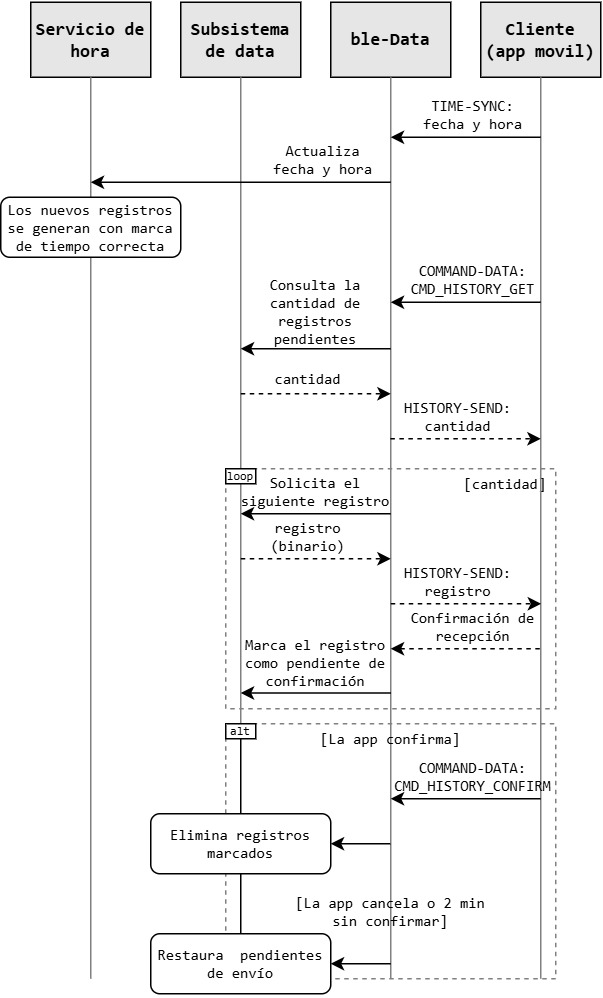
\includegraphics[width=0.62\textwidth]{Figures/historico.jpg}
\caption[Sincronización horaria y descarga del histórico]{Sincronización horaria y descarga transaccional del histórico. La aplicación primero actualiza la hora del equipo y luego descarga los registros pendientes, que se eliminan solo si confirma la descarga y se restauran si la cancela o no responde en dos minutos.}
\label{fig:flujo_historico}
\end{figure}

\subsection{Parámetros}
\label{subsec:integracion_parametros}

La configuración del N150 se administra mediante un gestor de parámetros preexistente, que ya atendía los cambios recibidos desde la plataforma. La interfaz BLE se integró con él mediante dos callbacks. El de lectura obtiene la configuración actual en el mismo formato JSON que el gestor genera para la plataforma, y la aplicación la solicita con el comando de lectura de parámetros. El de procesamiento recibe los cambios que la aplicación envía por \texttt{PARAMETROS-GET}, una vez reensamblados por \texttt{ble-rcvMsg}. El gestor valida y aplica cada cambio con las mismas reglas que utiliza para la plataforma, y su respuesta se devuelve a la aplicación por \texttt{PARAMETROS-RESPONSE}.

Luego de procesar un cambio recibido por BLE, el gestor deja pendiente un reporte forzado de la configuración, que la lógica de nube envía a la plataforma. Así, la plataforma conserva una copia actualizada de los parámetros, aunque el cambio no haya llegado por los canales remotos. La figura \ref{fig:flujo_parametros} muestra el recorrido completo de una escritura de parámetros. El propio componente aprovecha este mecanismo: \texttt{APP\_LINK} se registra en el gestor como un parámetro más, por lo que el modo de operación de la interfaz puede modificarse por los mismos medios que el resto de la configuración.

\begin{figure}[htbp]
\centering
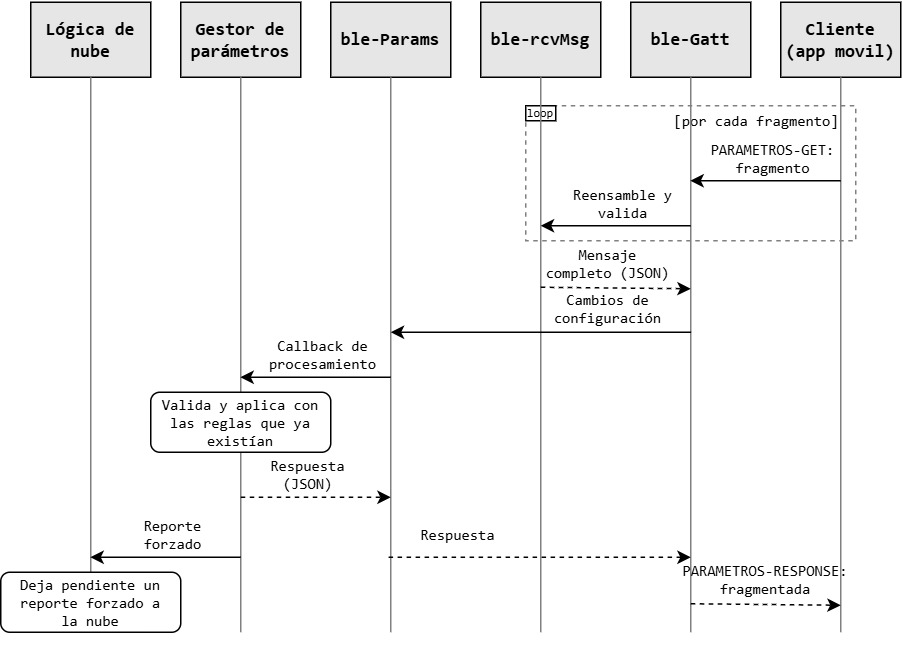
\includegraphics[width=\textwidth]{Figures/params.jpg}
\caption[Escritura de parámetros]{Escritura de parámetros desde la aplicación móvil. Los fragmentos recibidos se reensamblan, el gestor de parámetros valida y aplica los cambios con sus reglas existentes, la respuesta vuelve a la aplicación y queda pendiente un reporte forzado a la plataforma.}
\label{fig:flujo_parametros}
\end{figure}

\subsection{Pruebas de actuadores}
\label{subsec:integracion_pruebas}

Las pruebas de actuadores permiten que el técnico verifique en el lugar el funcionamiento de la heladera. Los comandos recibidos por \texttt{COMMAND-GET} se entregan mediante un callback a las rutinas de control existentes del N150, que habilitan el modo de prueba y accionan de forma individual el compresor, la resistencia, el ventilador y la luz, o ejecutan la rutina de prueba completa. El argumento del comando indica si la prueba se inicia o se detiene. El resultado que devuelve la rutina se informa a la aplicación por \texttt{COMMANDS-RESPONSE}. De este modo, la interfaz local no accede directamente a los actuadores, sino que utiliza las rutinas de prueba que el controlador ya tenía implementadas.

La figura \ref{fig:flujo_comando} muestra el recorrido genérico de un comando. Las lecturas de metadatos y diagnóstico, descritas a continuación, siguen el mismo recorrido, con la diferencia de que la solicitud llega por \texttt{COMMAND-DATA} y la respuesta se transmite fragmentada por indicaciones.

\begin{figure}[htbp]
\centering
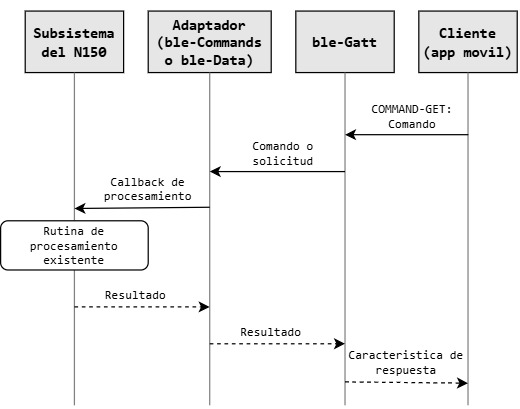
\includegraphics[width=0.7\textwidth]{Figures/comando.jpg}
\caption[Recorrido genérico de un comando]{Recorrido genérico de un comando. La solicitud se delega mediante un callback a la rutina existente del subsistema correspondiente, y el resultado vuelve a la aplicación por la característica de respuesta asociada.}
\label{fig:flujo_comando}
\end{figure}

\subsection{Metadatos y diagnóstico}
\label{subsec:integracion_metadatos}

Los metadatos y el diagnóstico se obtienen mediante callbacks que devuelven un documento JSON. Para los metadatos, el firmware reutiliza la información que la lógica de nube y conectividad remota ya construía para la plataforma, como el modelo y el serial del controlador, las versiones de firmware y los datos del módem y de la red celular. El diagnóstico reúne el estado de la conectividad del equipo, como la conexión activa, el registro en la red celular y la conexión con la plataforma, para que el técnico pueda identificar en el lugar por qué un equipo no reporta. En ambos casos, \texttt{ble-Data} copia el documento, \texttt{ble-Gatt} lo transmite fragmentado por indicaciones y el resultado de la operación se informa por \texttt{READ-STATUS}.

\subsection{Comandos para la lógica de nube y conectividad remota}
\label{subsec:integracion_nube}

Algunas operaciones, como la desactivación de la conectividad celular, ya existían como comandos que el N150 recibe desde la plataforma. Para no duplicarlas, la interfaz BLE acepta esos mismos comandos por \texttt{CLOUDCOMMANDS-GET}. El mensaje, en formato JSON, se reensambla y se entrega mediante un callback a la cola de comandos de la lógica de nube y conectividad remota. A partir de ese punto, el comando sigue el mismo camino de validación y ejecución que uno recibido de forma remota.

\subsection{Registros}
\label{subsec:integracion_registros}

La interfaz ofrece tres canales de registros, que se activan cuando la aplicación se suscribe a la característica correspondiente. \texttt{LOG-SEND} toma las entradas de la cola del sistema de registros del N150 y las transmite con el formato JSON de ese sistema. \texttt{LOG-TERMINAL} intercepta la salida de terminal del firmware mientras la aplicación está suscrita y la almacena en un búfer circular de 64 entradas de hasta 256 bytes, ubicado en la PSRAM cuando está disponible; si el búfer se llena, se descartan las entradas más antiguas. Por último, \texttt{LOG-CONTROL} es un canal independiente que los módulos del firmware pueden utilizar para informar eventos y el estado de un proceso en curso, sin consumir la cola general de registros.

Estos canales permiten observar el comportamiento del N150 durante una intervención de soporte sin depender de la conectividad celular ni de una conexión física a la terminal del equipo.
